\documentclass[11pt, a4paper]{scrartcl}

\usepackage{fullpage}
\usepackage{listings}
\usepackage{graphicx}


\newcommand{\email}[1]{\small{#1}}
\newcommand{\cname}[1]{\mbox{\texttt{#1}}}

\title{Programming of Parallel Computers}
\subtitle{Assignment 2. PThreads.}
\author{Christos Sakalis \\ \email{Christos.Sakalis.3822@student.uu.se}
    \and Aliaksandr Ivanou \\ \email{Aliaksandr.Ivanou.1364@student.uu.se}}

\begin{document}

\maketitle

\section{Introduction}

In this report we present the results that we got by running pthread implementations.

\section{Results}

There were several experiments. The figure \ref{fig:ct} shows the dependence of execution time on the amount of threads. The size of input data is 100000000. The figure \ref{fig:st} shows the dependence of the size. The number of threads is 20.

As we can see the builtin sort produces the expected output. The time almost the same for different number of cores, also there is linear dependence on size.

The Devide and Conquer algorithm showed quite good results. Until approximately 10 threads, this algorithm shows good scalability. But after 10 threads, it has almost the same execution time. The DNC algorithm has a tree structure. At each iteration current thread creates two new threads with the smaller arrays and waits their execution. With a large input array and a large number of threads we will have a lot of threads that are just waiting and doing nothing. This can be the obstacle for DNC algorithm. 

The Peer sorting algorithm behaved strangely. As can be seen, it scales well until ~12 threads, but then the execution time raises. Each iteration there only halve of threads running. It can be one of performance obstacles. This algorithm is similar to odd-even sort. Here, we have the same problem: load imbalance. But, using pthreads we are eliminating unnecessary communication and data exchange.

The parallel quicksort has a best performance. We can see, that the execution time decreases with the amount of threads. 

Also, during tests there were other programms running and possibly could affect results.

\begin{figure}
    \centering
    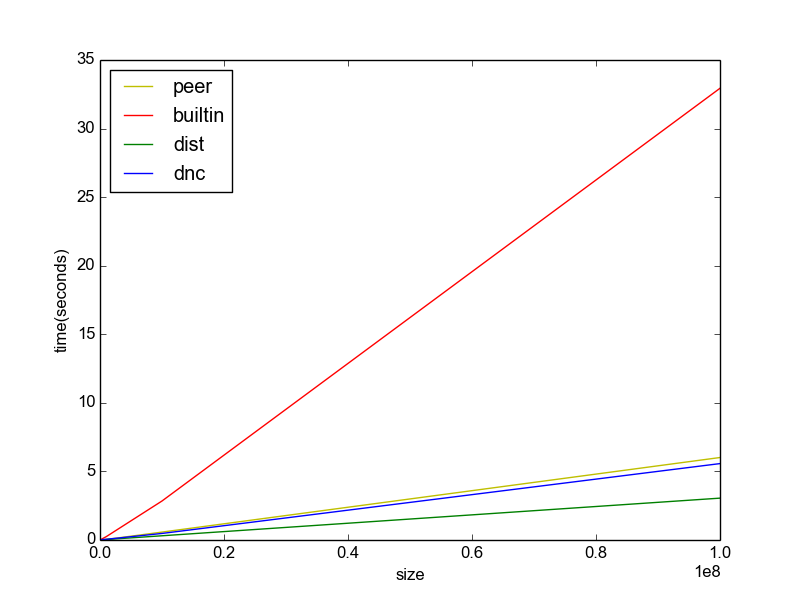
\includegraphics[scale=0.6]{size_time.png}
    \caption{Size - time dependence}
    \label{fig:st}
\end{figure}

\begin{figure}
    \centering
    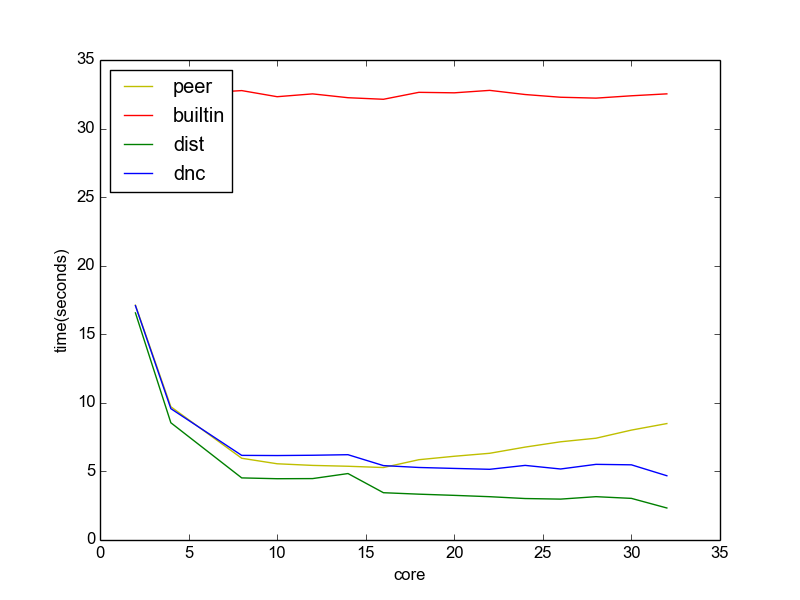
\includegraphics[scale=0.6]{core_time.png}
    \caption{Core - time dependence}
    \label{fig:ct}
\end{figure}


\section{The code}


\lstinputlisting{qsort_chris.c}


\end{document}
